\documentclass[11pt]{article}
\usepackage{anysize}
\marginsize{1.2cm}{1.4cm}{.4cm}{1cm}

\usepackage[normalem]{ulem}
\usepackage{amsfonts}
\usepackage{amsmath}
\usepackage[shortlabels]{enumitem}
\usepackage[font=small,labelfont=bf]{caption}
\usepackage{graphicx}
\usepackage{listings}
\lstset{
  basicstyle=\ttfamily,
  mathescape
}

\setlength{\parindent}{0pt}

\newcommand{\by}{\mathbf{y}}
\newcommand{\bY}{\mathbf{Y}}
\newcommand{\bX}{\mathbf{X}}
\newcommand{\btheta}{\mathbf{\theta}}
\newcommand{\bI}{\mathbf{I}}
\newcommand{\bA}{\mathbf{A}}
\newcommand{\bB}{\mathbf{B}}
\newcommand{\bW}{\mathbf{W}}

\newcommand{\thh}{\hat{\theta}}
\newcommand{\yh}{\hat{y}}
\newcommand{\sgn}{\text{ sign}}
\DeclareMathOperator*{\argmin}{arg\,min}
\newcommand{\pcd}{\text{PATHWISE\_CD}}

\begin{document}

\begin{center}
\textbf{Exploring Regularization Techniques for Small Data Sets} \\
Ian Dardik, Heeru Ahuja \\
CS6140 \\
\end{center}

\section{Introduction}
In this paper we focus on regularization techniques that improve linear regression modeling on small data sets.  The classic Ordinary Least Squares (OLS) method becomes numerically unstable as the number of samples decrease, and has no solution when the number of parameters exceed the sample size.  Statistical regularization can be applied to help stabilize the solution to a linear regeression problem and make modeling feasible for small data sets.  In this paper we will explore and compare several options for building a regularized linear regression model in the context of a data set whose sample size is small compared to the number of parameters.  

\section{Methods}
Statistical regularization helps stabilize our model and reduce the variance, which becomes increasingly important as the number of samples shrink.  Unforunatley, regularization introduces bias into our model so we must choose an appropriate balance.  The models we consider in this paper control the degree of regularization through one or two tuning parameters that are completely suppressed at zero, and influence our model more as they increase towards infinity.  We can estimate the ideal tuning parameter values by using cross-validation to estimate the Mean Squared Error (MSE) for a small universe of tuning parameters, and select the parameters that minimize MSE.  Each regularization technique that we consider is formulated as an optimization problem that minimizes an objective function $J$ of the form:
	$$\thh = \argmin\limits_\theta J(\theta) =\argmin\limits_\theta \sum\limits_{i=1}^N L(\theta) + \sum\limits_{i=1}^P R(\theta,\lambda)$$

Where $L(\theta)$ is the loss function and $R(\theta,\lambda)$ is the regularization rule that depends on the tuning parameter $\lambda$, and sometimes an additional tuning parameter $\alpha$.  We often refer to the regularization rule as the \textit{penalty}.  We only consider squared loss in this paper, i.e. $L(\theta)= (Y_i - X_i'\theta)^2$, however we consider and discuss several options for choice of the regularization rule.  The regularization techniques that we consider are:
\begin{itemize}
	\item L1 penalty (LASSO)
	\item L2 penalty (Ridge)
	\item Elastic Net
	\item L2 with Custom Soft-Thresholding
	\item L$\frac{1}{2}$ penalty (not included in our Results section)
\end{itemize}

Many of the regularization techniques we discuss do not have a closed analytical solution, so we will consider two algorithms for numerically arriving at a solution: Batch Gradient Descent and Pathwise Coordinate Descent.  The following sections detail how to use each regularization rule with each algorithm.  \\

For the remainder of this paper we assume that all data $X$ and responses $Y$ are standardized.  

\subsection{Gradient Descent}
Gradient Descent algorithms work by moving in the direction that the gradient of $\theta$ points, with distance scaled by a learning rate parameter $\alpha$.  The algorithm continuously updates it value for the parameter vector $\theta$ until convergence.  Gradients point towards local optima, so we clearly need to use convex objective functions to arrive at a gobally optimal solution in Gradient Descent.  Fortunately, computing the gradient of objective functions listed above is straightforward which makes Gradient Descent fairly simple to implement.  Notice that Gradient Descent works by computing the gradient; it does not itself solve an optimization problem per se; since the algorithm is only dependent on the gradient of the objective function, we can parameterize it based on the gradient.  Therefore we end up with a core algorithm the form: $\text{GRADIENT\_DESCENT}(\nabla\theta)$

\subsection{Pathwise Coordinate Descent}
While Gradient Descent operates on the entire parameter vector at once, Pathwise Coordinate Descent (PCD) concentrates on each parameter individually.  Pathwise Coordinate Descent considers each parameter $\theta_j$ as its own optimization problem\cite{ht}:
	$$\thh_j = \argmin\limits_{\theta_j} J(\theta)$$

In each iteration of the PCD algorithm, we update each $\theta_j$ to be the solution to the individual optimization problem.  

\subsubsection{Parameterizing the PCD Algorithm}
Pathwise Coordinate Descent is parameterized by the objective function $J$ that it solves for each $\theta_j$.  However, for the universe of objective functions we consider in this paper, we can parameterize the PCD algorithm by just two nonnegative parameters we call $A$ and $B$.  For each objective function we consider below, we will show that the solution to optimizing each $\theta_j$ takes the form:
	$$\theta_j = S\left(\sum\limits_{i=1}^N X_{ij}(Y_i - \sum\limits_{k \ne j}^p X_{ik}\theta_k), B\right)/A$$

Where we define\cite{ht} $S(t,B) = \sgn(t)(|t|-B)_+$, and $()_+$ is the soft-thresholding operator.  It follows that each algorithm reduces to the following parameterized form $\pcd(A, B)$.  In the following sections we will show how each of the objective functions we consider fit into this parameterization.  

\subsubsection{LASSO}
LASSO uses the L1 norm for a penalty:
	$$\thh_j = \argmin\limits_{\theta_j} \frac{1}{2} \sum\limits_{i=1}^N \left(Y_i - \sum\limits_{k=1}^px_{ik}\theta_k \right)^2 + \lambda \sum\limits_{k=1}^p|\theta_k|$$

Where $\lambda \geq 0$ is a tuning parameter.  Let $J$ be the objective function we want to optimize above.  We can solve for $\theta_j$ by finding the stationary points of $J$:
\begin{equation}\begin{split}
	\frac{\partial J}{\partial \theta_j}
		& = -\sum\limits_{i=1}^N X_{ij}(Y_i - X_{ij}\theta_j - \sum\limits_{k \ne j}^p X_{ik}\theta_k) + \lambda \sgn(\theta_j) \\
		& = -\sum\limits_{i=1}^N X_{ij}(Y_i - \sum\limits_{k \ne j}^p X_{ik}\theta_k) + \sum\limits_{i=1}^NX_{ij}^2\theta_j + \lambda \sgn(\theta_j) \\
		& = -\sum\limits_{i=1}^N X_{ij}(Y_i - \sum\limits_{k \ne j}^p X_{ik}\theta_k) +(N-1)\theta_j + \lambda \sgn(\theta_j) \\
\end{split}\end{equation}

The last step follows from the fact that our data is standardized, and thus $\sum\limits_{i=1}^NX_{ij}^2 = N-1$.  \\

Set $\frac{\partial J}{\partial \theta_j}=0$ and, for convenience, let $Q = \sum\limits_{i=1}^N X_{ij}(Y_i - \sum\limits_{k \ne j}^p X_{ik}\theta_k)$ and and we get:
	$$(N-1)\theta_j + \lambda\sgn(\theta_j) = Q$$

To solve for $\theta_j$ notice that when $\theta_j \geq 0$, $\theta_j=\frac{Q-\lambda}{N-1}$ so $Q \geq \lambda$.  However when $\theta_j \leq 0$, $\theta_j=\frac{Q+\lambda}{N-1}$ so $Q \leq -\lambda$.  Notice the following two properties: \\
	\hspace*{1cm} (1) $|Q| \geq \lambda$ \\
	\hspace*{1cm} (2) $\theta_j \geq 0$ iff $Q \geq 0$ and $\theta_j \leq 0$ iff $Q \leq 0$ \\

Therefore, we can write the solution for $\theta_j$ as:
	$$\theta_j = \frac{\sgn(Q)(|Q|-\lambda)_+}{N-1}$$

Where the soft-thresholding operator guarantees property (1), while multiplying by $\sgn(Q)$ makes use of (and guarantees) property (2).  Recall that $S(t,B) = \sgn(t)(|t|-B)_+$, then our final solution is:
	$$\theta_j = S\left(\sum\limits_{i=1}^N X_{ij}(Y_i - \sum\limits_{k \ne j}^p X_{ik}\theta_k), \lambda\right)/(N-1)$$

Notice this yields a solution nearly identical to Elements of Statistical Learning\cite{ht}; the difference is that we divide by $N-1$ and we believe this is likely a typo in the book.  \\

Notice that the soft-thresholding parameter is $\lambda$; this explains why larger $\lambda$ values causes LASSO to drive parameter values to zero.  It is now clear that LASSO performs subset selection due to the choice of regularization penalty \textit{and} algorithm.  \\

Finally, it is clear that the parameterization for LASSO is $\pcd(N-1,\lambda)$.  


\subsubsection{Elastic Net}
The Elastic Net uses the tuning parameter $\alpha \in [0,1]$ to compromise between Ridge and Lasso penalization.  Ridge penalizes the L2 norm, so Elastic Net solves the following optimization problem:
	$$\thh_j = \argmin\limits_{\theta_j} \frac{1}{2} \sum\limits_{i=1}^N \left(Y_i - \sum\limits_{k=1}^px_{ik}\theta_k \right)^2 + \lambda \sum\limits_{k=1}^p \left(\alpha\theta_k^2 + (1-\alpha)|\theta_k| \right)$$

This math is very similar to LASSO above so we have left the details to the appendix.  Our final solution is:
	$$\theta_j = S\left(\sum\limits_{i=1}^N X_{ij}(Y_i - \sum\limits_{k \ne j}^p X_{ik}\theta_k), B\right)/A$$

Where $A=(N-1)+2\lambda\alpha$, and $B=\lambda(1-\alpha)$.  This equation is already in our desired form, and hence the parameterization is $\pcd(N-1+2\lambda\alpha,\lambda(1-\alpha))$.  

\subsubsection{Ridge}
Ridge Regularization has a closed form analytical solution so it does not require an algorithm.  Nevertheless, we will discuss Ridge in the context of PCD to realize why the L2 penalty does not perform subset selection while the L1 does.  We can simply use our solution for the Elastic Net with $\alpha=1$ for the Ridge solution.  This implies that $A=(N-1)+2\lambda$ and $B=0$, yielding:
	$$\theta_j = S\left(\sum\limits_{i=1}^N X_{ij}(Y_i - \sum\limits_{k \ne j}^p X_{ik}\theta_k), 0\right)/(N-1+2\lambda)$$

With parameterization $\pcd(N-1+2\lambda,0)$.  Notice that the soft-thresholding parameter is zero; this implies that \textit{no} soft-thresholding will be applied for Ridge, regardless of the parameter $\lambda$.  This explains why Ridge tends to shrink parameter values but doesn't drive them towards zero.  

\subsubsection{Custom Shrinkage Methods}
\label{csm}
We have found above that LASSO uses $\lambda$ exclusively for linear shrinkage and soft-thresholding, while Ridge uses $\lambda$ exclusively for inverse shrinkage.  The Elastic Net implicitly combines both shrinkage techniques using two tuning parameters; here we propose three ``custom" ideas for combining the shrinkage types using a single tuning parameter.  Our hope is that using a single tuning parameter makes it easier to find the optimal bias-variance tradeoff using cross-validation.  These custom ideas, inspired by Nearest Shrunken Centroids, apply soft-thresholding to the Ridge solution in the form: $\pcd(N-1 + 2\lambda, STP(\lambda))$, where $STP$ is the soft-thresholding penalty function.  The three custom ideas we will explore are:
\begin{enumerate}
	\item Ridge with Soft-Thresholding: $\pcd(N-1 + 2\lambda, \lambda)$
	\item Ridge with Quadratic Soft-Thresholding: $\pcd(N-1 + 2\lambda, \lambda^2)$
	\item Ridge with Exponential Soft-Thresholding: $\pcd(N-1 + 2\lambda, e^\lambda-1)$
\end{enumerate}

\subsection{Experimental Design}
In order to compare each regularization technique, we generated two data sets on which we trained and tested our suite of algorithms.  Our models include 27 individual parameters, where $X_0 ... X_{25}$ are continuous and $X_{26}$ is a categorical variable representing a month of the year.  The first model includes four orthogonal design variables:
	$$m_{ortho}(X) = 2X_1 + 3X_7^2 + 4X_8 + 2X_{37} + \epsilon_{ortho}$$

Where $\epsilon_{ortho} \sim \mathcal{N}(0,4)$.  Our second model includes two design variables that are each correlated with two parameters:
	$$m_{corr}(X) = 2X_1^3I_{Dec}(X_{26}) + 3X_{23}X_{24} + \epsilon_{corr}$$

Where $\epsilon_{corr} \sim \mathcal{N}(0,1)$, and the indicator $I_{Dec}$ is one if the given argument is ``Dec" and zero otherwise.  For both data sets we generated four sets of samples:
\begin{enumerate}
	\item ``$n<p$": a training data set where the number of samples is smaller than the number of parameters.  We chose 20 samples.  
	\item ``$n=p$": a training data set where the number of samples is approximately equal to the number of parameters  We chose 40 samples even though we have 38 variables in our design matrix.  We use 5-fold cross-valdiation in which we require the number of samples to be divisble by 5; hence the choice of 40 samples.  
	\item ``$n>p$": a training data set where the number of samples exceeds the number of parameters.  We chose 80 samples; we purposely chose a number of samples that exceeds the number of parameters, but is still relatively small.  
	\item ``Test": a testing data set with a large number of samples for estimating the Mean Squared Error (MSE) of the fitted model.  We chose 10,000 samples.  
\end{enumerate}

For each data set, we trained each algorithm using a design matrix that is linear in each of the 26 continuous variables, and included 12 extra indicator variables for the categorical month variable.  We chose optimal tuning parameters for each algorithm using 5-fold cross-validation and then computed the test MSE on the ``Test" data set.  Our results are included in the following section.  


\section{Results}
For each algorithm, we have included the Test MSE, parameter subset selection, and the number of correctly and incorrectly selected parameters.  In addition, we have included three columns comparing each algorithm to the sklearn library results, where we subtract our implementation value from the library value.  We have the following remarks on our results:
\begin{itemize}
	\item Our LASSO implementation and sklearn have similar performance based on Test MSE.  The margin is small, but our implementation outperforms the library on the orthogonal data set in the $n<p$ and $n>p$ case.  
	\item Our algorithms generally outperform the library in terms of subset selection.  In particular, Ridge with Exponential Soft-Thresholding either beats or ties the library in subset selection for every case, and does so by a decent margin in the orthogonal case.  
	\item Both our algorithms and the library performed poorly on the correlated data set.  
	\item LASSO with Batch Gradient Descent performed very poorly on subset selection, which is completely expected by the choice of algorithm.  
\end{itemize}

\begin{center}
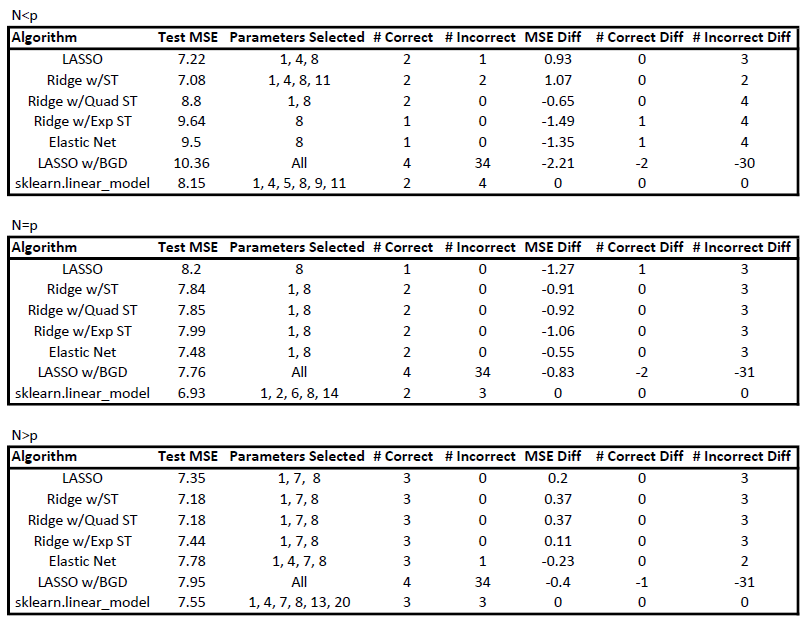
\includegraphics[scale=0.7]{ortho.PNG}
\captionof{figure}{Orthogonal Dataset Results}
\end{center}

\begin{center}
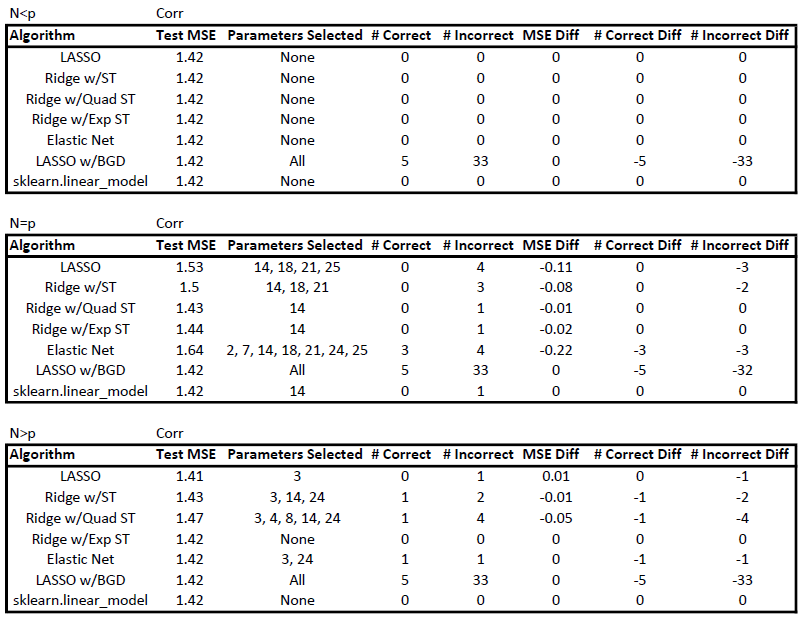
\includegraphics[scale=0.7]{corr.PNG}
\captionof{figure}{Correlated Dataset Results}
\end{center}


\section{Discussion}
While the main focus of this paper is on comparing regularization techniques, it is worth noting that our data suggests that some form of regularization is important to stabilize linear regression.  In section \ref{cvtr}, the training error graphs in figures 4, 8, 12, 13, 16 and 26 show how the MSE can spike as regularization approaches zero, while the training error graphs in figures 3, 10, 24 and 25 show how the MSE can become highly volitile as regularization approaches zero.  \\

Our results do not show a clear choice of algorithm that minimizes prediction error on our data sets.  However, Ridge with Exponential Soft-Thresholding does stand out as the best performing algorithm in terms of subset selection.  Unfortunately our experimental data is narrow in scope--using just two data sets, one of which saw poor performances across all algorithms--thus more testing is necessary before drawing any conclusions about Ridge with Exponential Soft-Thresholding.  There may be merrit in continuing to experiment with this technique: the training error graphs in figures 21, 22, and 23 of section \ref{cvtr} suggest that we may not have considered the optimal tuning parameter.  The algorithms can take a long time to converge as regularization decreases, making it tough to test all of our desired options of tuning parameters.  \\

More generally, it is not clear that any of the custom shrinkage methods we proposed are worthwhile.  However it is worth noting that squashing linear/soft-thresholding and inverse shrinkage into a single tuning parameter has a clear advantage: it is easier to implement.  While Elastic Net also combines linear/soft-thresholding and inverse shrinkage into a single regularization technique, we found that it was slightly easier to implement cross-validation for a single tuning parameter and \textit{far} easier to graph the results for a single tuning parameter.  We experimented with 3D graps to no avail; we ended up plotting Elastic Net as a function of $\alpha$ values, choosing the best $\lambda$ value at each value of $\alpha$ (see section \ref{cvtr} figures 27-32).  \\

We have also found that choosing tuning parameters via cross-validation alone is not necessarily easy.  Our graphs clearly show that training error is not a convex function of tuning parameters, however our analysis would have benefited greatly from a more robust method of choosing our tuning parameters.  \\

Finally, it is worth noting that implementing the algorithms--particularly PCD--was not trivial.  Understanding PCD requires understanding the optimization problem that each regularization technique uses; this was not trivial at first but led to many key insights, including the custom shrinkage methods from section \ref{csm}.  


\begin{thebibliography}{9}
\bibitem{ht}
Trevor Hastie, Robert Tibshirani, and Jerome Friedman,
The Elements of Statistical Learning 2nd Edition

\bibitem{tib}
Tibshirani's paper
\end{thebibliography}

\section{Appendix}

\subsection{Github Repository}

\subsection{Elastic Net Derivation}

\subsection{$L\frac{1}{2}$ Norm Derivation}

\subsection{Cross-Validation Training Results}
\label{cvtr}
\begin{center}
% LASSO
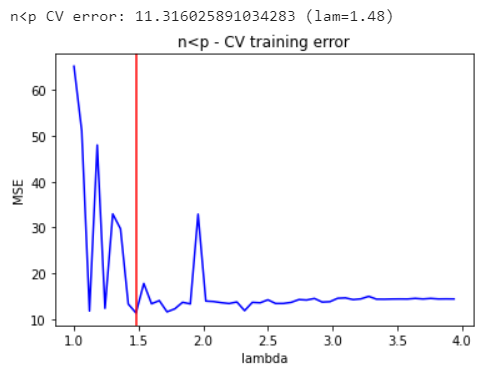
\includegraphics[scale=0.7]{charts/lasso_ortho_n_lt_p_err.PNG}
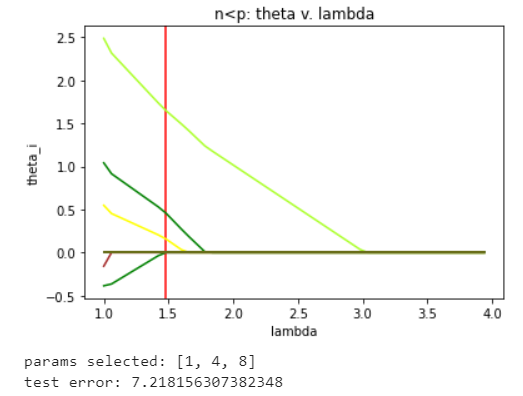
\includegraphics[scale=0.7]{charts/lasso_ortho_n_lt_p_thetas.PNG}
\captionof{figure}{LASSO, $n<p$ orthogonal data set}

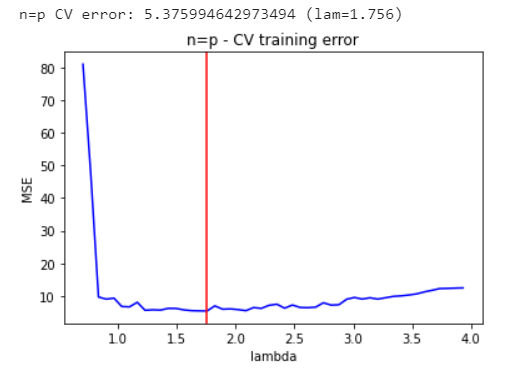
\includegraphics[scale=0.7]{charts/lasso_ortho_n_eq_p_err.PNG}
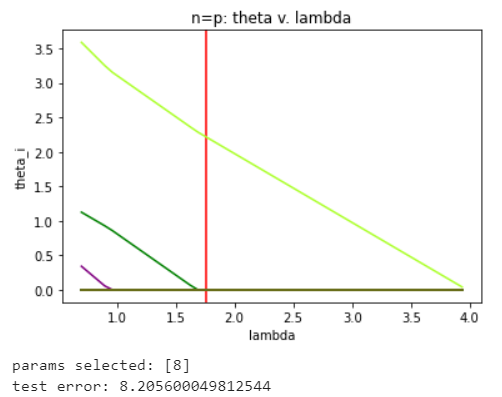
\includegraphics[scale=0.7]{charts/lasso_ortho_n_eq_p_thetas.PNG}
\captionof{figure}{LASSO, $n=p$ orthogonal data set}

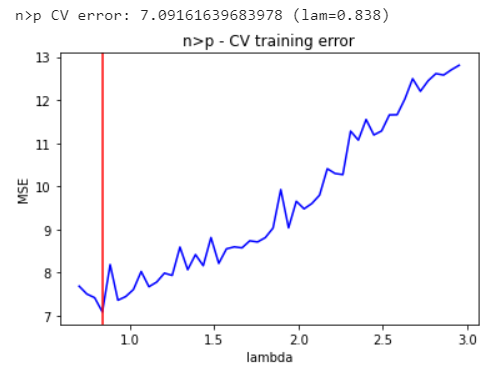
\includegraphics[scale=0.7]{charts/lasso_ortho_n_gt_p_err.PNG}
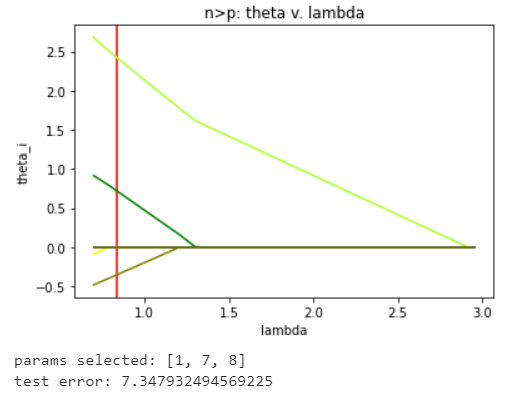
\includegraphics[scale=0.7]{charts/lasso_ortho_n_gt_p_thetas.PNG}
\captionof{figure}{LASSO, $n>p$ orthogonal data set}

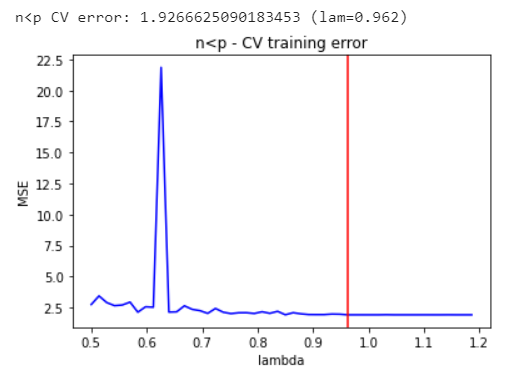
\includegraphics[scale=0.7]{charts/lasso_corr_n_lt_p_err.PNG}
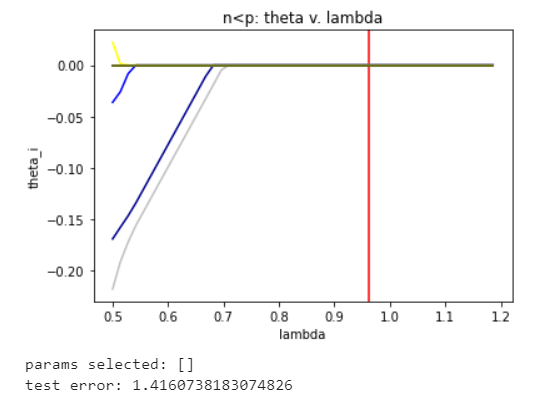
\includegraphics[scale=0.7]{charts/lasso_corr_n_lt_p_thetas.PNG}
\captionof{figure}{LASSO, $n<p$ correlated data set}

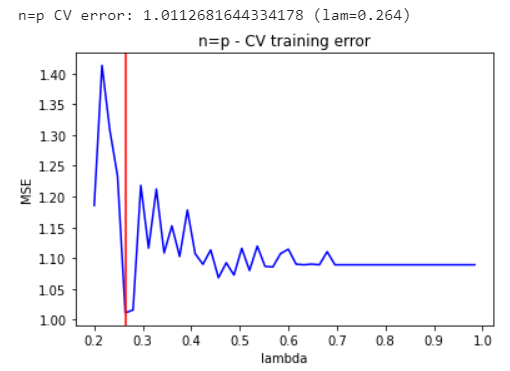
\includegraphics[scale=0.7]{charts/lasso_corr_n_eq_p_err.PNG}
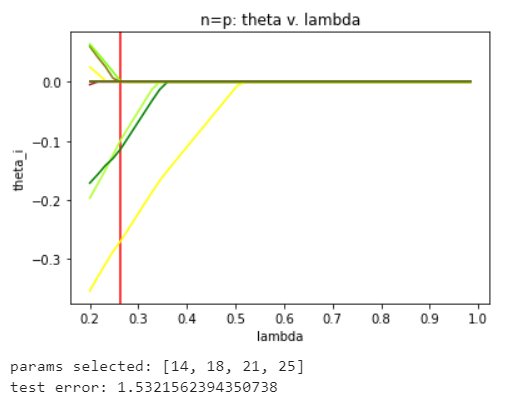
\includegraphics[scale=0.7]{charts/lasso_corr_n_eq_p_thetas.PNG}
\captionof{figure}{LASSO, $n=p$ correlated data set}

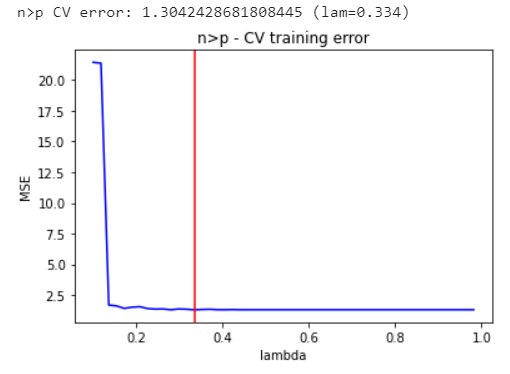
\includegraphics[scale=0.7]{charts/lasso_corr_n_gt_p_err.PNG}
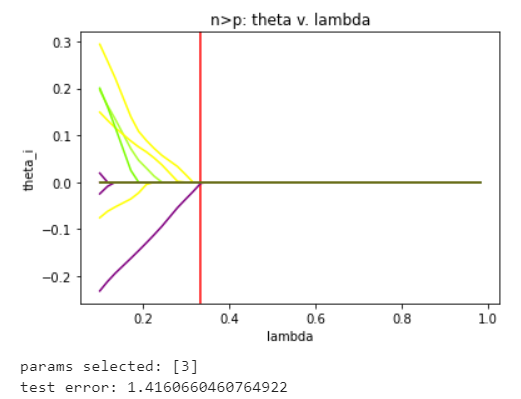
\includegraphics[scale=0.7]{charts/lasso_corr_n_gt_p_thetas.PNG}
\captionof{figure}{LASSO, $n>p$ correlated data set}

% Ridge w/ST
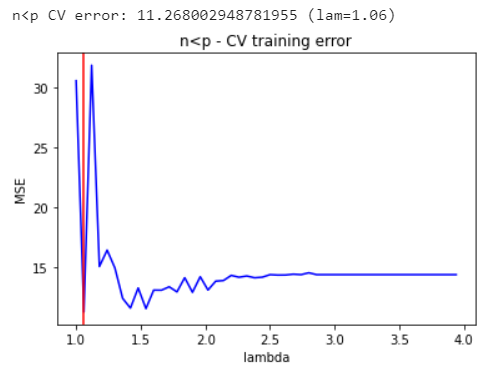
\includegraphics[scale=0.7]{charts/ridge_st_ortho_n_lt_p_err.PNG}
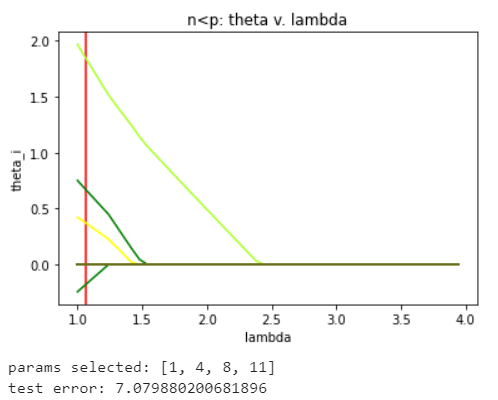
\includegraphics[scale=0.7]{charts/ridge_st_ortho_n_lt_p_thetas.PNG}
\captionof{figure}{Ridge with Soft-Thresholding, $n<p$ orthogonal data set}

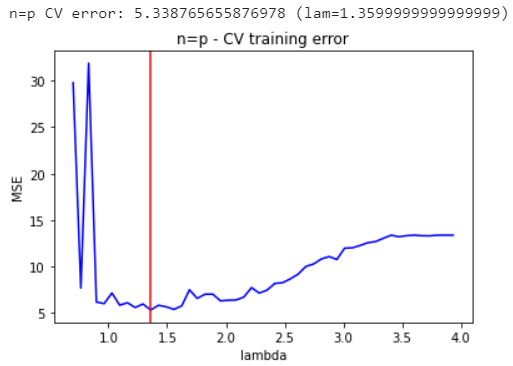
\includegraphics[scale=0.7]{charts/ridge_st_ortho_n_eq_p_err.PNG}
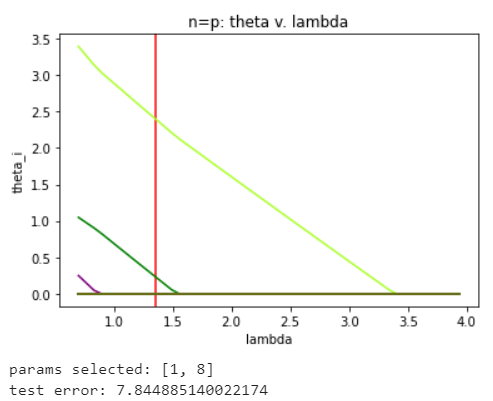
\includegraphics[scale=0.7]{charts/ridge_st_ortho_n_eq_p_thetas.PNG}
\captionof{figure}{Ridge with Soft-Thresholding, $n=p$ orthogonal data set}

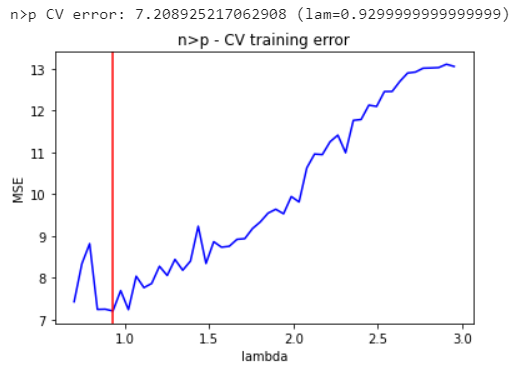
\includegraphics[scale=0.7]{charts/ridge_st_ortho_n_gt_p_err.PNG}
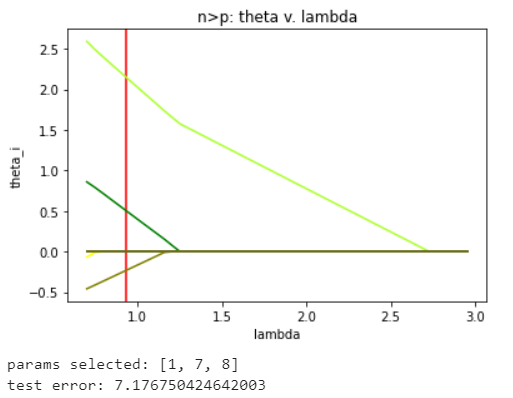
\includegraphics[scale=0.7]{charts/ridge_st_ortho_n_gt_p_thetas.PNG}
\captionof{figure}{Ridge with Soft-Thresholding, $n>p$ orthogonal data set}

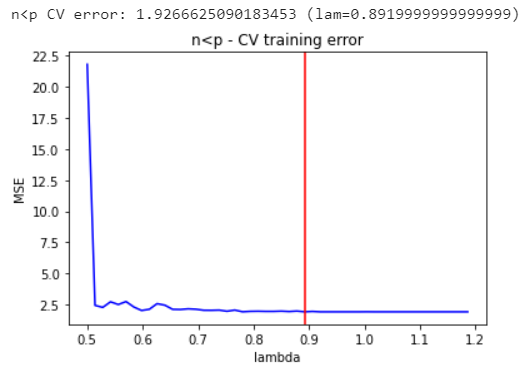
\includegraphics[scale=0.7]{charts/ridge_st_corr_n_lt_p_err.PNG}
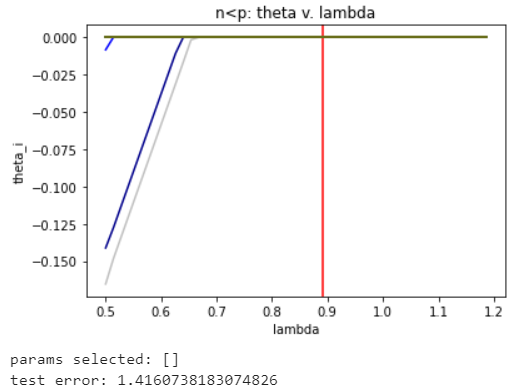
\includegraphics[scale=0.7]{charts/ridge_st_corr_n_lt_p_thetas.PNG}
\captionof{figure}{Ridge with Soft-Thresholding, $n<p$ correlated data set}

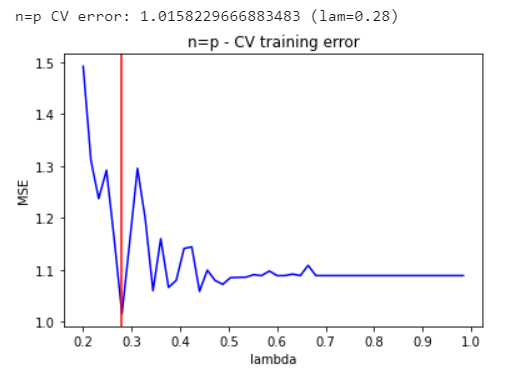
\includegraphics[scale=0.7]{charts/ridge_st_corr_n_eq_p_err.PNG}
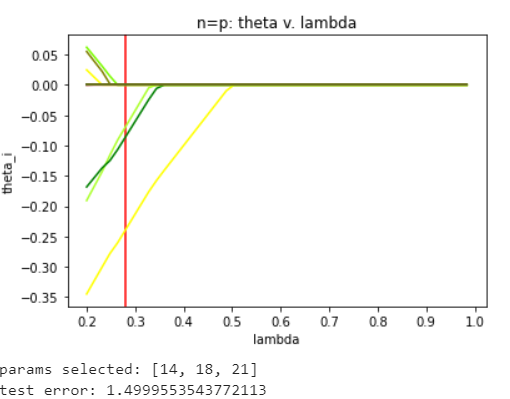
\includegraphics[scale=0.7]{charts/ridge_st_corr_n_eq_p_thetas.PNG}
\captionof{figure}{Ridge with Soft-Thresholding, $n=p$ correlated data set}

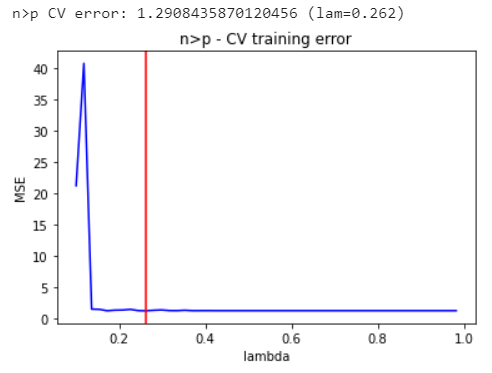
\includegraphics[scale=0.7]{charts/ridge_st_corr_n_gt_p_err.PNG}
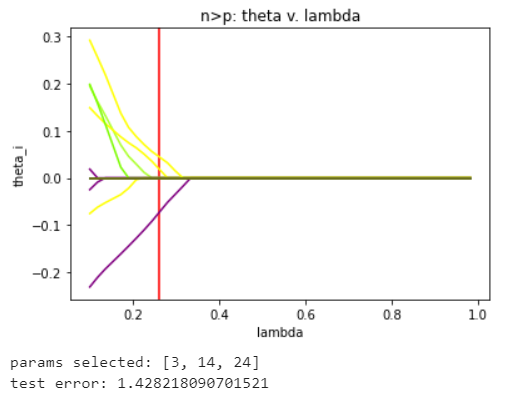
\includegraphics[scale=0.7]{charts/ridge_st_corr_n_gt_p_thetas.PNG}
\captionof{figure}{Ridge with Soft-Thresholding, $n>p$ correlated data set}

% Ridge w/Q ST
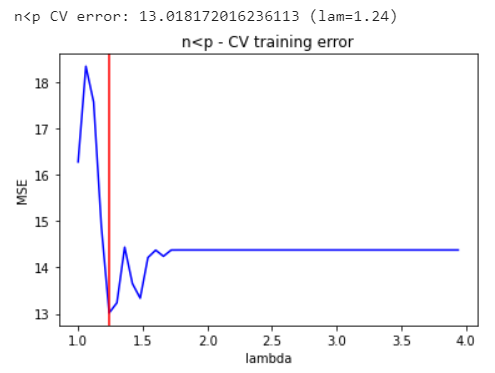
\includegraphics[scale=0.7]{charts/ridge_q_ortho_n_lt_p_err.PNG}
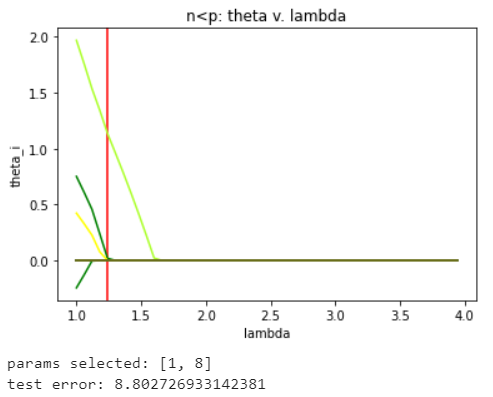
\includegraphics[scale=0.7]{charts/ridge_q_ortho_n_lt_p_thetas.PNG}
\captionof{figure}{Ridge with Quadratic Soft-Thresholding, $n<p$ orthogonal data set}

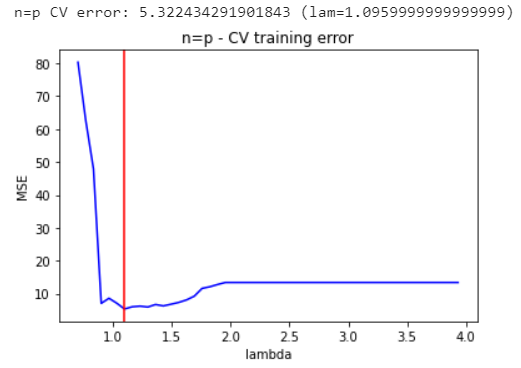
\includegraphics[scale=0.7]{charts/ridge_q_ortho_n_eq_p_err.PNG}
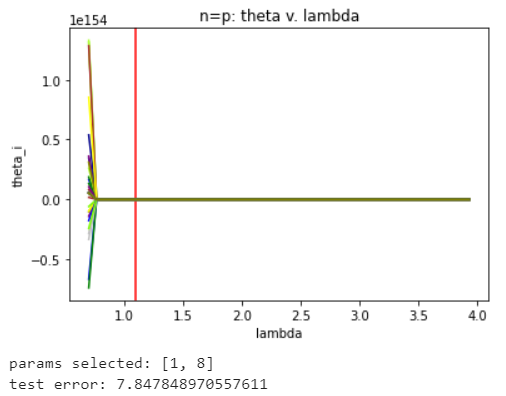
\includegraphics[scale=0.7]{charts/ridge_q_ortho_n_eq_p_thetas.PNG}
\captionof{figure}{Ridge with Quadratic Soft-Thresholding, $n=p$ orthogonal data set}

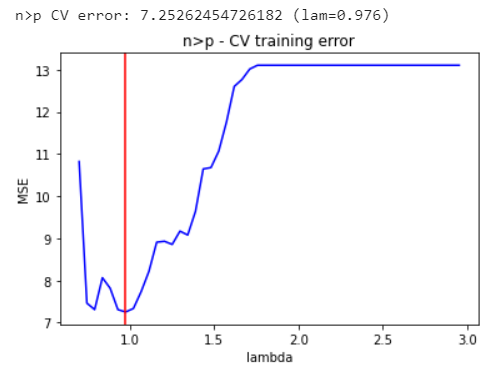
\includegraphics[scale=0.7]{charts/ridge_q_ortho_n_gt_p_err.PNG}
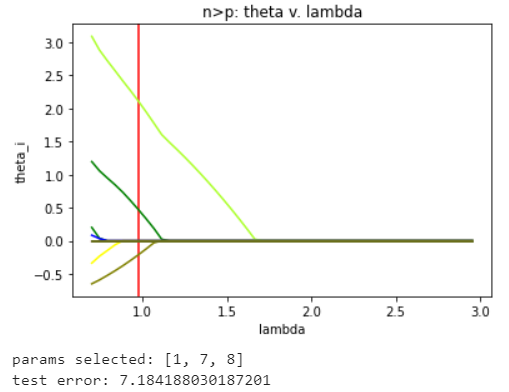
\includegraphics[scale=0.7]{charts/ridge_q_ortho_n_gt_p_thetas.PNG}
\captionof{figure}{Ridge with Quadratic Soft-Thresholding, $n>p$ orthogonal data set}

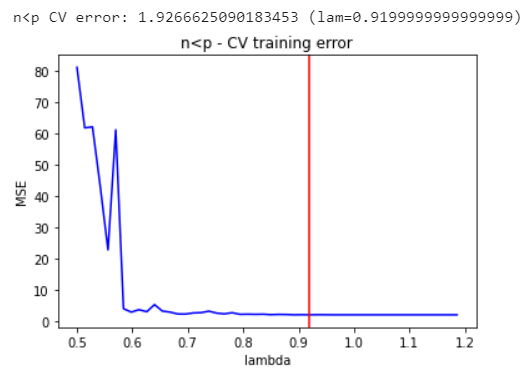
\includegraphics[scale=0.7]{charts/ridge_q_corr_n_lt_p_err.PNG}
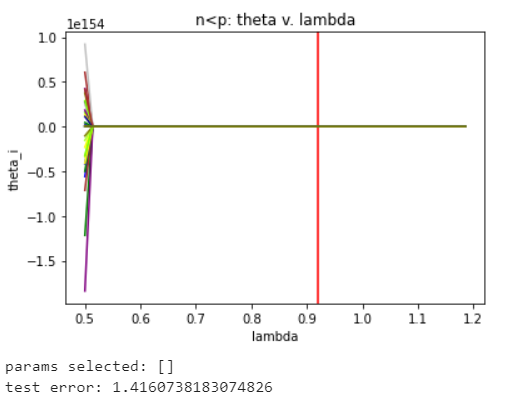
\includegraphics[scale=0.7]{charts/ridge_q_corr_n_lt_p_thetas.PNG}
\captionof{figure}{Ridge with Quadratic Soft-Thresholding, $n<p$ correlated data set}

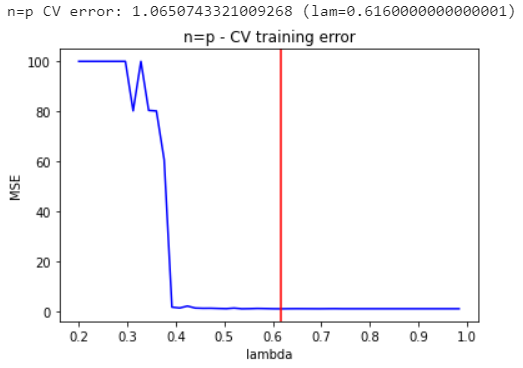
\includegraphics[scale=0.7]{charts/ridge_q_corr_n_eq_p_err.PNG}
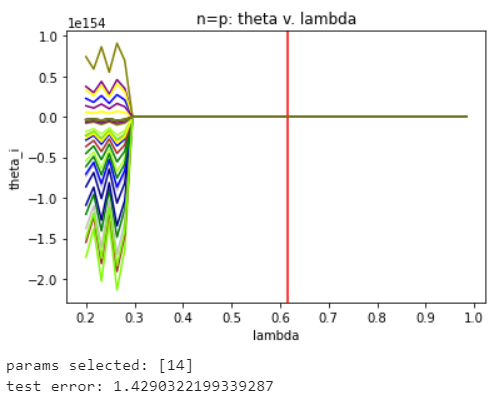
\includegraphics[scale=0.7]{charts/ridge_q_corr_n_eq_p_thetas.PNG}
\captionof{figure}{Ridge with Quadratic Soft-Thresholding, $n=p$ correlated data set}

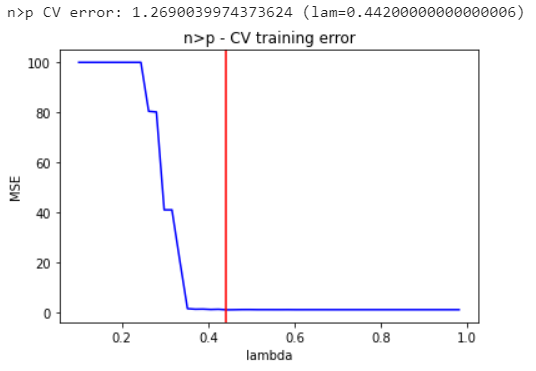
\includegraphics[scale=0.7]{charts/ridge_q_corr_n_gt_p_err.PNG}
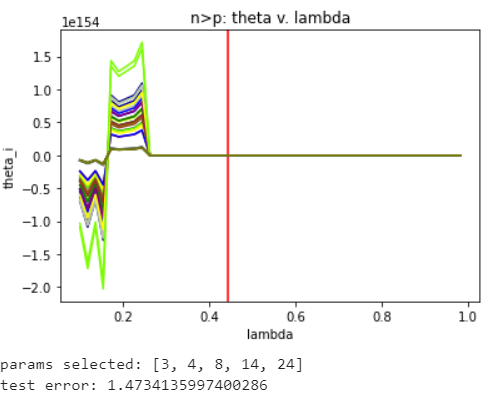
\includegraphics[scale=0.7]{charts/ridge_q_corr_n_gt_p_thetas.PNG}
\captionof{figure}{Ridge with Quadratic Soft-Thresholding, $n>p$ correlated data set}

% Ridge w/Exp ST
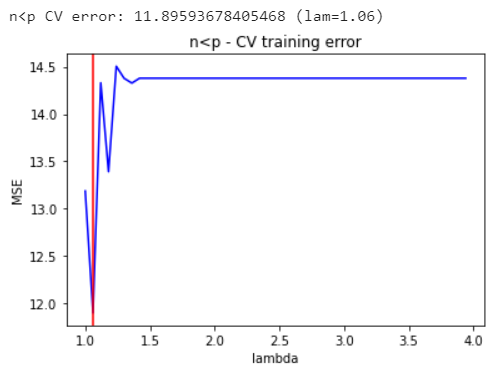
\includegraphics[scale=0.7]{charts/ridge_exp_ortho_n_lt_p_err.PNG}
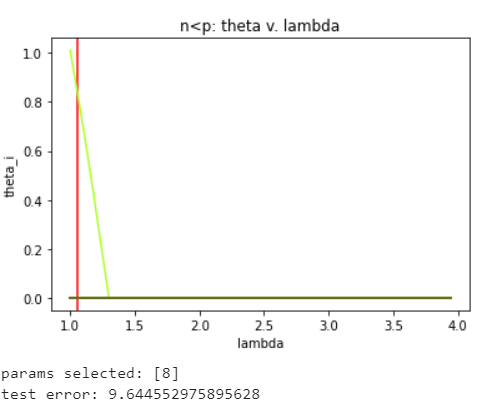
\includegraphics[scale=0.7]{charts/ridge_exp_ortho_n_lt_p_thetas.PNG}
\captionof{figure}{Ridge with Exponential Soft-Thresholding, $n<p$ orthogonal data set}

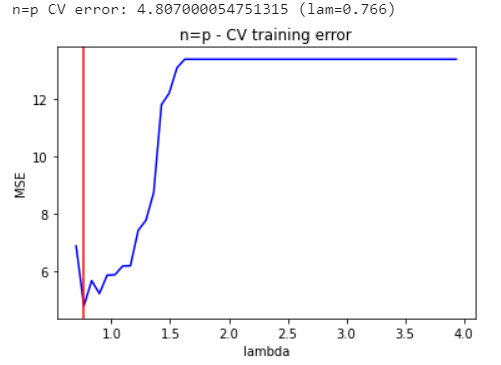
\includegraphics[scale=0.7]{charts/ridge_exp_ortho_n_eq_p_err.PNG}
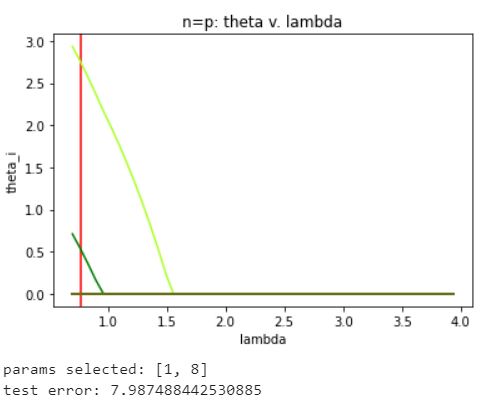
\includegraphics[scale=0.7]{charts/ridge_exp_ortho_n_eq_p_thetas.PNG}
\captionof{figure}{Ridge with Exponential Soft-Thresholding, $n=p$ orthogonal data set}

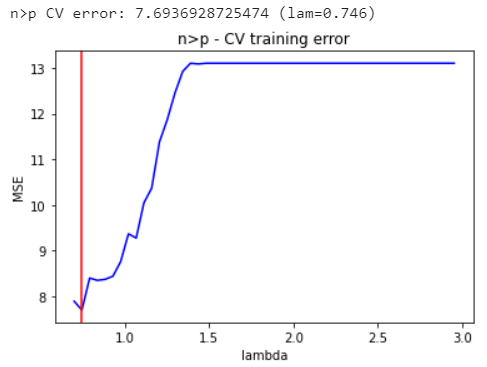
\includegraphics[scale=0.7]{charts/ridge_exp_ortho_n_gt_p_err.PNG}
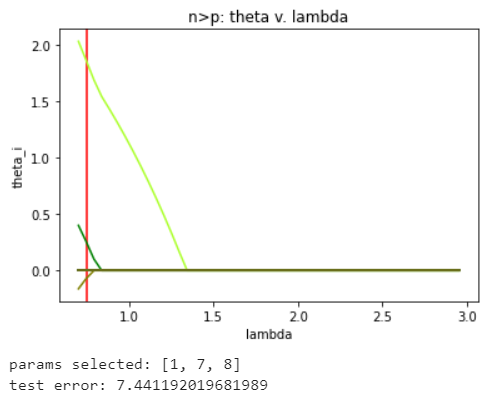
\includegraphics[scale=0.7]{charts/ridge_exp_ortho_n_gt_p_thetas.PNG}
\captionof{figure}{Ridge with Exponential Soft-Thresholding, $n>p$ orthogonal data set}

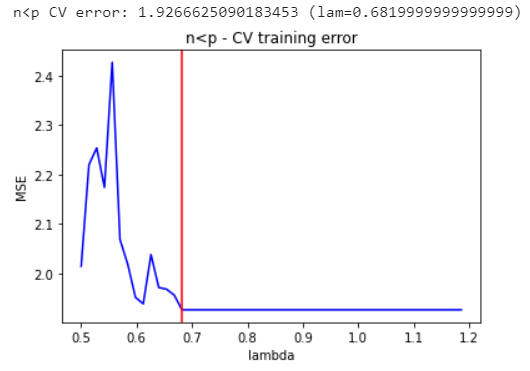
\includegraphics[scale=0.7]{charts/ridge_exp_corr_n_lt_p_err.PNG}
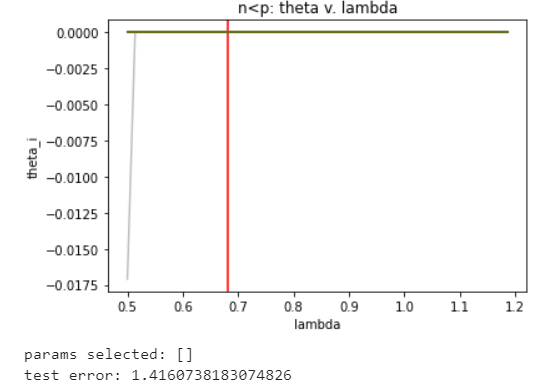
\includegraphics[scale=0.7]{charts/ridge_exp_corr_n_lt_p_thetas.PNG}
\captionof{figure}{Ridge with Exponential Soft-Thresholding, $n<p$ correlated data set}

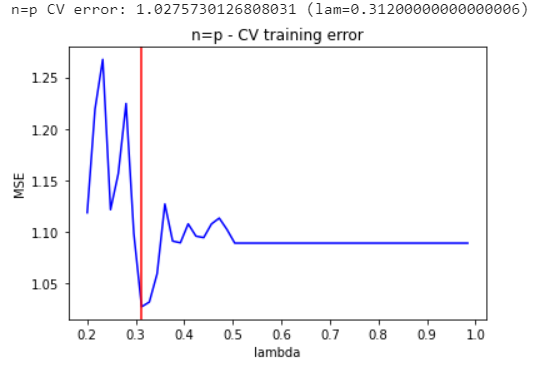
\includegraphics[scale=0.7]{charts/ridge_exp_corr_n_eq_p_err.PNG}
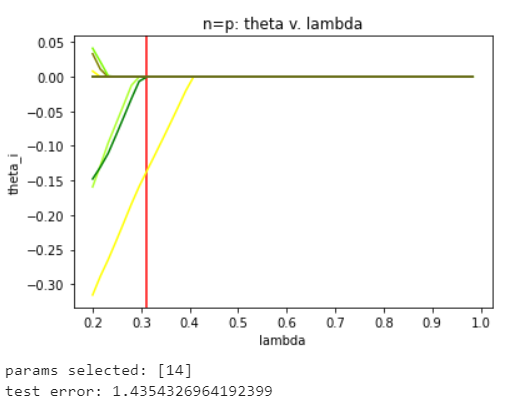
\includegraphics[scale=0.7]{charts/ridge_exp_corr_n_eq_p_thetas.PNG}
\captionof{figure}{Ridge with Exponential Soft-Thresholding, $n=p$ correlated data set}

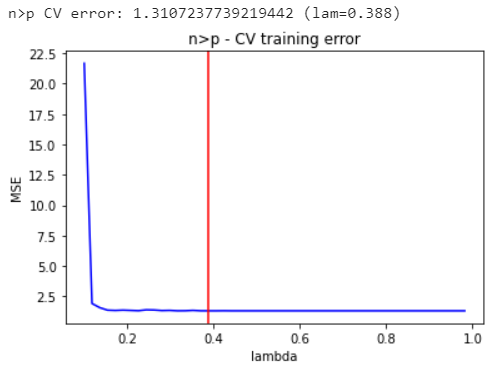
\includegraphics[scale=0.7]{charts/ridge_exp_corr_n_gt_p_err.PNG}
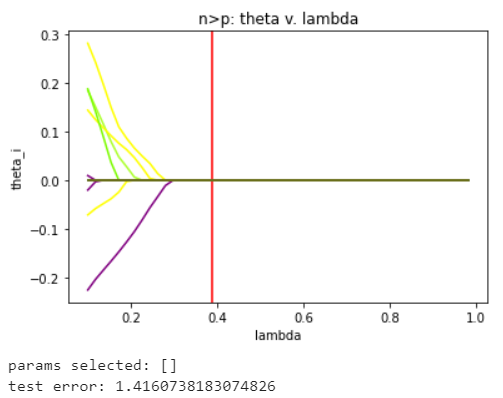
\includegraphics[scale=0.7]{charts/ridge_exp_corr_n_gt_p_thetas.PNG}
\captionof{figure}{Ridge with Exponential Soft-Thresholding, $n>p$ correlated data set}

% Elastic Net
\includegraphics[scale=0.7]{charts/en_ortho_n_lt_p_err.PNG}
\includegraphics[scale=0.7]{charts/en_ortho_n_lt_p_thetas.PNG}
\captionof{figure}{Elastic Net, $n<p$ orthogonal data set}

\includegraphics[scale=0.7]{charts/en_ortho_n_eq_p_err.PNG}
\includegraphics[scale=0.7]{charts/en_ortho_n_eq_p_thetas.PNG}
\captionof{figure}{Elastic Net, $n=p$ orthogonal data set}

\includegraphics[scale=0.7]{charts/en_ortho_n_gt_p_err.PNG}
\includegraphics[scale=0.7]{charts/en_ortho_n_gt_p_thetas.PNG}
\captionof{figure}{Elastic Net, $n>p$ orthogonal data set}

\includegraphics[scale=0.7]{charts/en_corr_n_lt_p_err.PNG}
\includegraphics[scale=0.7]{charts/en_corr_n_lt_p_thetas.PNG}
\captionof{figure}{Elastic Net, $n<p$ correlated data set}

\includegraphics[scale=0.7]{charts/en_corr_n_eq_p_err.PNG}
\includegraphics[scale=0.7]{charts/en_corr_n_eq_p_thetas.PNG}
\captionof{figure}{Elastic Net, $n=p$ correlated data set}

\includegraphics[scale=0.7]{charts/en_corr_n_gt_p_err.PNG}
\includegraphics[scale=0.7]{charts/en_corr_n_gt_p_thetas.PNG}
\captionof{figure}{Elastic Net, $n>p$ correlated data set}

% Elastic Net
\includegraphics[scale=0.7]{charts/bgd_ortho_n_lt_p_err.PNG}
\includegraphics[scale=0.7]{charts/bgd_ortho_n_lt_p_thetas.PNG}
\captionof{figure}{LASSO with Batch Gradient Descent, $n<p$ orthogonal data set}

\includegraphics[scale=0.7]{charts/bgd_ortho_n_eq_p_err.PNG}
\includegraphics[scale=0.7]{charts/bgd_ortho_n_eq_p_thetas.PNG}
\captionof{figure}{LASSO with Batch Gradient Descent, $n=p$ orthogonal data set}

\includegraphics[scale=0.7]{charts/bgd_ortho_n_gt_p_err.PNG}
\includegraphics[scale=0.7]{charts/bgd_ortho_n_gt_p_thetas.PNG}
\captionof{figure}{LASSO with Batch Gradient Descent, $n>p$ orthogonal data set}

\includegraphics[scale=0.7]{charts/bgd_corr_n_lt_p_err.PNG}
\includegraphics[scale=0.7]{charts/bgd_corr_n_lt_p_thetas.PNG}
\captionof{figure}{LASSO with Batch Gradient Descent, $n<p$ correlated data set}

\includegraphics[scale=0.7]{charts/bgd_corr_n_eq_p_err.PNG}
\includegraphics[scale=0.7]{charts/bgd_corr_n_eq_p_thetas.PNG}
\captionof{figure}{LASSO with Batch Gradient Descent, $n=p$ correlated data set}

\includegraphics[scale=0.7]{charts/bgd_corr_n_gt_p_err.PNG}
\includegraphics[scale=0.7]{charts/bgd_corr_n_gt_p_thetas.PNG}
\captionof{figure}{LASSO with Batch Gradient Descent, $n>p$ correlated data set}
\end{center}

\end{document}














